\section{Einführung in die Regelaufgabe} \label{sec:Einfuehrung}

Photovoltaikanlagen enthalten viele Tausend einzelne Photovoltaikzellen. Jede einzelne wandelt einfallende Sonnenstrahlung (direkt und indirekt) in elektrischen Strom um. Unter Vernachlässigung von Verlusten in Kabeln, Wandlerverlusten und Leistungsfehlanpassungen ist die erzeugte Leistung von PV-Systemen die Anzahl aller enthaltenen Zellen multipliziert mit der Leistung einer einzelnen Zelle. Über diese Annahme ist es möglich das das mathematische Modell der gesamten PV-Anlage für die Systemanalyse abzuleiten. \\
Die Grundeinheiten einer PV-Anlage sind die PV-Module oder auch Solarzellen. Ein Standard-PV-Modul besteht aus 48 bis 73 in Reihe geschalteten Zellen, die in einen Rahmen montiert sind. PV-Anlagen werden in der Regel durch Reihen- und Parallelschaltungen von Modulen zusammengesetzt. Solarmodule werden in Reihe geschaltet (sog.\xspace \glqq Strings\grqq{}), um die Ausgangsspannung zu erhöhen. Parallel geschaltete Strings bilden ein \glqq Array\grqq{}, in dem die Leistungskapazität von Tausenden bis Millionen Watt aufgebaut werden kann. \\
Das mathematische Modell des PV-Generators ergibt sich aus der Zusammenfassung aller PV-Module, die durch das Modell einer einzelnen Zelle beschrieben werden, wobei Strom und Spannung in geeigneter Weise multipliziert werden .Dazu wird die Einzelzelle durch ein Ersatzschaltbild modelliert, das aus einer einstrahlungsabhängigen Stromquelle, einem Modell der Diode $D$ und Shunt-Widerstand $R_{\mathrm{h}}$ besteht, wie in \autoref{fig:Bild1} (links) dargestellt. Die Einstrahlung $S$ mit der physikalischen Einheit $\SI{}{\frac{W}{m^2}}$ bezieht sich auf die direkte (normal zum PV-Zellenfeld) und die indirekte Einstrahlung. \\
\newline
Um die Spannung von PV-Anlagen zu regeln, werden Gleichspannungswandler eingesetzt. Die Ausgangsspannung des Wandlers kann eingestellt werden und unterscheidet sich von der Eingangsspannung. Eine grundlegende Gleichspannungswandlerschaltung ist der so genannte Buck Converter (Tiefsetzsteller), welcher ebenfalls in \autoref{fig:Bild1} (rechts) dargestellt ist. \\
Die Pulsweitenmodulation (PWM) ermöglicht die Steuerung und Regelung der gesamten Ausgangsspannung. Die PWM stellt ein Rechtecksignal bereit, welches zwischen 0 und 1 schaltet. Typische Schaltfrequenzen liegen zwischen $f_{\mathrm{SW}} = \SI{1}{kHz} \ldots \SI{1}{MHz}$. Im Falle der konkreten Anlage beträgt die Schaltfrequenz $f_{\mathrm{SW}} = \SI{5}{kHz}$. In der Praxis werden \zB MOSFET's als Schalter eingesetzt. Die Ausgangsspannung hinter dem MOSFET (siehe ebenfalls \autoref{fig:Bild1} (mittig)) wechselt somit zwischen Null und der Ausgangsspannung des Wandlers $v_{\mathrm{DC}}$. Das Tastverhältnis (Duty Cycle) $d$ beschreibt die Zeitverhältnisse des Rechtecksignals, also somit wann der Schalter (MOSFET) in Position 0 \bzw 1 ist. Der Duty Cycle lässt sich wie folgt berechnen:

\begin{align}
    d = \frac{v_{\mathrm{DC}}}{v_{\mathrm{PV}}} \quad \text{\bzw} \quad d = \frac{i_{\mathrm{PV}}}{i_{\mathrm{DC}}}
    \label{eq:Gleichung1}
\end{align}

Nachfolgend findet sich die Darstellung der Modellparameter/Konstanten zur Modellierung des Buck Converters (siehe \autoref{tab:Tabelle1}).

\begin{table}[H]
    \centering
    \begin{tabular}{|lll|}
        \hline
        \rowcolor{grey}
        \textbf{Symbol}          & \textbf{Parameter}                               & \textbf{Wert}                            \\ \hline
        \rowcolor{lightGrey}
        \multicolumn{3}{|c|}{Standard Testbedingungen (STC)}                                                                   \\ \hline
        $T_{\mathrm{c,STC}}$     & PV Zelltemperatur bei STC                        & $\SI{298}{K}$                            \\
        $S_{\mathrm{STC}}$       & Bestrahlung bei STC                              & $\SI{1000}{\frac{W}{m^2}}$               \\
        $v_{\mathrm{T,STC}}$     & Thermische Spannung der p-n Sperrschicht bei STC & $\SI{25.7 \cdot 10^{-3}}{V}$             \\
        $i_{\mathrm{ph,sc,STC}}$ & Kurzschlussstrom des Diodenmodells bei STC       & $\SI{9.272}{A}$                          \\
        $v_{\mathrm{oc,STC}}$    & Leerlaufspannung bei STC                         & $\SI{0.644}{V}$                          \\ \hline
        \rowcolor{lightGrey}
        \multicolumn{3}{|c|}{Maximaler Leistungspunkt (MPP)}                                                                   \\ \hline
        $i_{\mathrm{PV,MPP}}$    & Gesamtstrom des PV Parks beim MPP                & $\SI{2902.13}{A}$                        \\
        $v_{\mathrm{PV,MPP}}$    & Gesamtspannung des PV Parks beim MPP             & $\SI{1049.13}{V}$                        \\
        $P_{\mathrm{MPP}}$       & Gesamtleistung des PV Parks beim MPP             & $\SI{30447.11}{W}$                       \\ \hline
        \rowcolor{lightGrey}
        \multicolumn{3}{|c|}{Weitere Parameter}                                                                                \\ \hline
        $R_{\mathrm{h}}$         & Shunt-Widerstand im Einzeldiodenmodell           & $\SI{10.196}{\Omega}$                    \\
        $v_{\mathrm{DC}}$        & Ausgangsgleichspannung                           & $\SI{900}{V}$                            \\
        $N_{\mathrm{cell,p}}$    & Anzahl paralleler Zellen pro Modul               & 1                                        \\
        $N_{\mathrm{cell,s}}$    & Anzahl serieller Zellen pro Modul                & 72                                       \\
        $N_{\mathrm{mod,p}}$     & Anzahl paralleler Module pro Anlage              & 336                                      \\
        $N_{\mathrm{mod,s}}$     & Anzahl serieller Module pro Anlage               & 27                                       \\
        $N_{\mathrm{p}}$         & Anzahl paralleler Zellen pro Anlage              & $\SI{336}{}$                             \\
        $N_{\mathrm{s}}$         & Anzahl serieller Zellen pro Anlage               & $\SI{1944}{}$                            \\
        $k$                      & Boltzmann Konstante                              & $\SI{1.381 \cdot 10^{-23}}{\frac{J}{K}}$ \\
        $q$                      & Elementarladung                                  & $\SI{1.602 \cdot 10^{-19}}{C}$           \\
        $A_{\mathrm{n}}$         & Dioden-Idealitätsfaktor im Einzeldiodenmodell    & $\SI{1.374}{}$                           \\
        $\alpha _{\mathrm{T}}$   & Temperaturkoeffizient des PV-Stroms              & $\SI{0.06 \cdot 10^{-2}}{}$              \\
        $\beta _{\mathrm{T}}$    & Temperaturkoeffizient der PV-Spannung            & $\SI{-0.36 \cdot 10^{-2}}{}$             \\ \hline
    \end{tabular}
    \caption{Modellparameter des Buck Converters}
    \label{tab:Tabelle1}
\end{table}

Ziel der Regelung soll es sein, die Ausgangsspannung $v_{\mathrm{DC}}$ konstant bei $\SI{900}{V}$ zu halten. Die einzelnen PV-Zellen wurden im Vorhinein messtechnisch analysiert für verschiedene Bestrahlungen und Temperaturen. Die nachfolgende Modellierung erfolgt zunächst für eine konstante Bestrahlung mit $S = \SI{1000}{\frac{W}{m^2}}$ bei einer konstanten Zelltemperatur von $T_{\mathrm{c}} = \SI{298}{K}$.

\begin{figure}[H]
   \centering
   \fbox{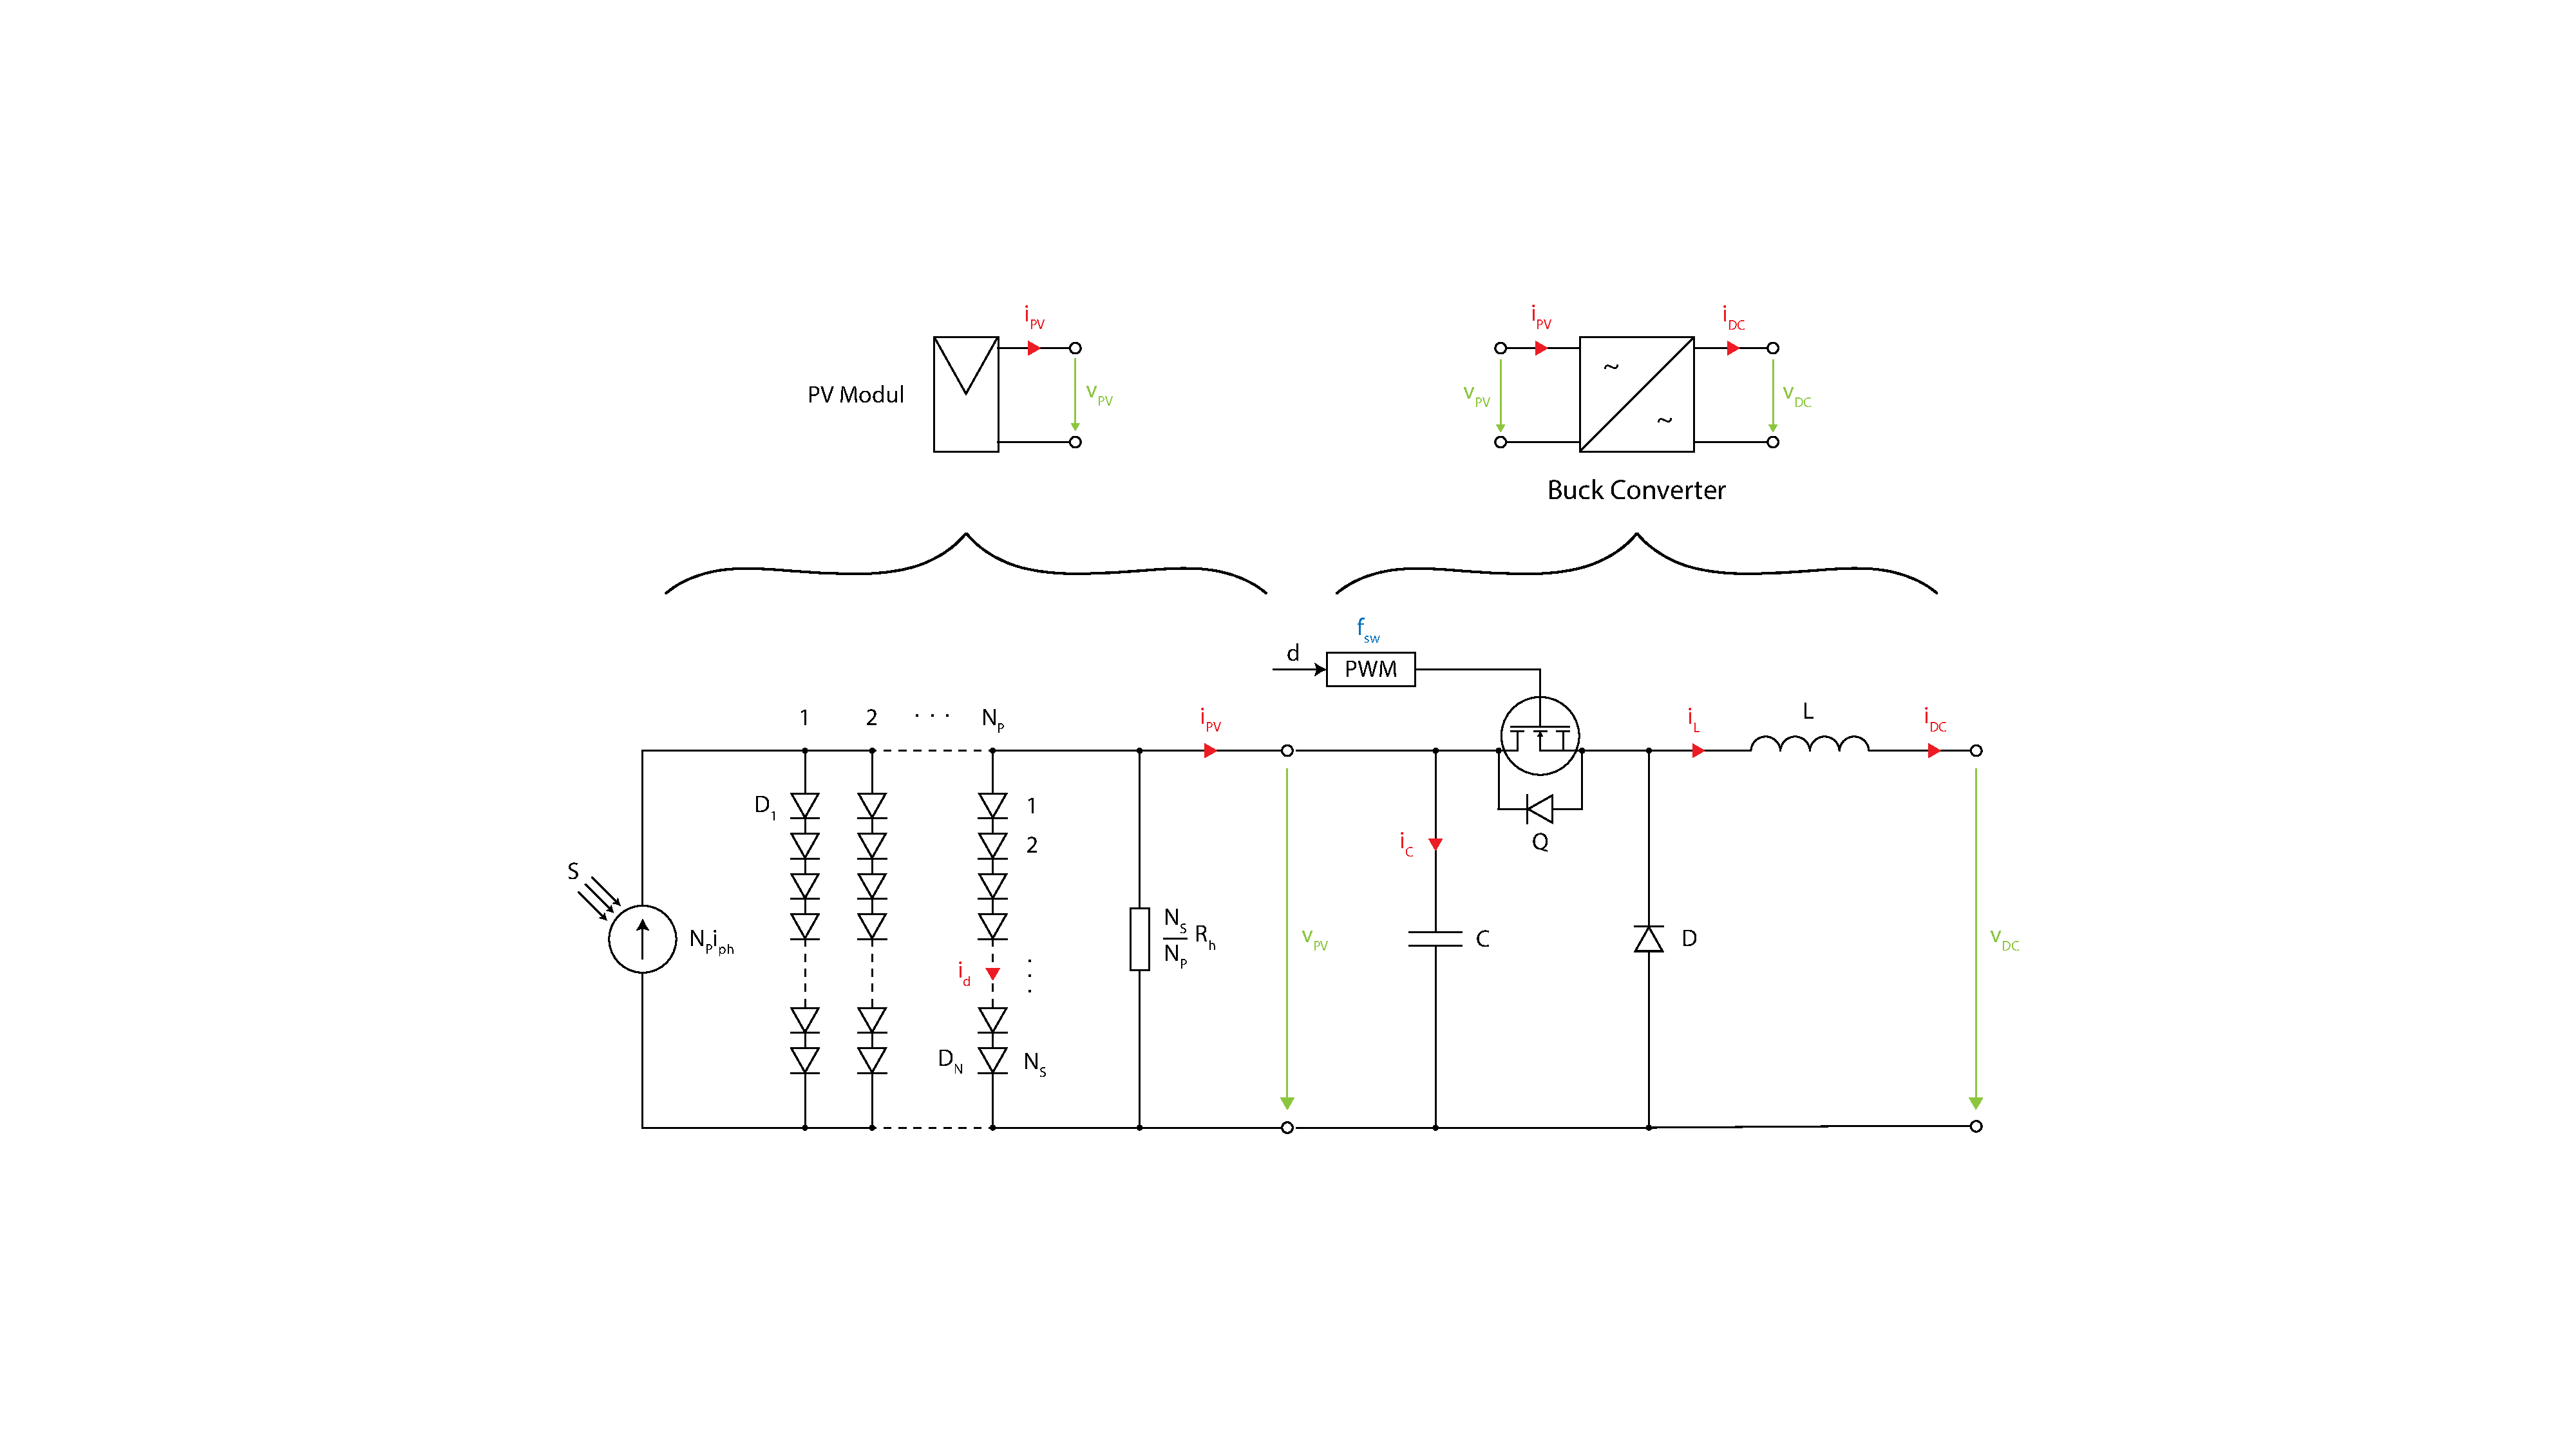
\includegraphics[width=1.0\textwidth]{Bilder/Buck_Zeichnung.pdf}}
   \caption[Skizze der Regelaufgabe]{Übersichtsschaltbild des Buck Converters als zu regelndes System inklusive Photovoltaik Anlage}
   \label{fig:Bild1}
\end{figure}